\section{Introdução}
\label{sec:introducao}

\subsection*{Definição}
%{\usebackgroundtemplate{\includegraphics[width=\paperwidth]{iot.jpg}}}
\begin{frame}{}
	\begin{block}{Internet}	
		Um vasto conjunto de redes diferentes que utilizam certos \textbf{protocolos} comuns e fornecem determinados \textbf{serviços} comuns \cite{tanenbaum2011computer}. 
	\end{block}
	
	\begin{figure}[H]
		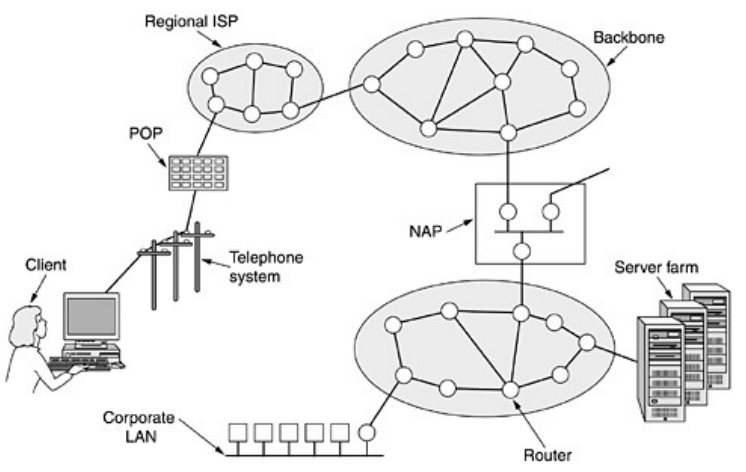
\includegraphics[width=.6\textwidth]{internet.png}\footnotemark
	\end{figure}
	
	\footnotetext{\cite{tanenbaum2011computer}}
\end{frame}

\begin{frame}{}
	\begin{block}{Coisa}	
		Tudo o que existe ou possa existir, de natureza corpórea ou incorpórea \cite{Michaelis}.
	\end{block}
	
	\begin{figure}[H]
		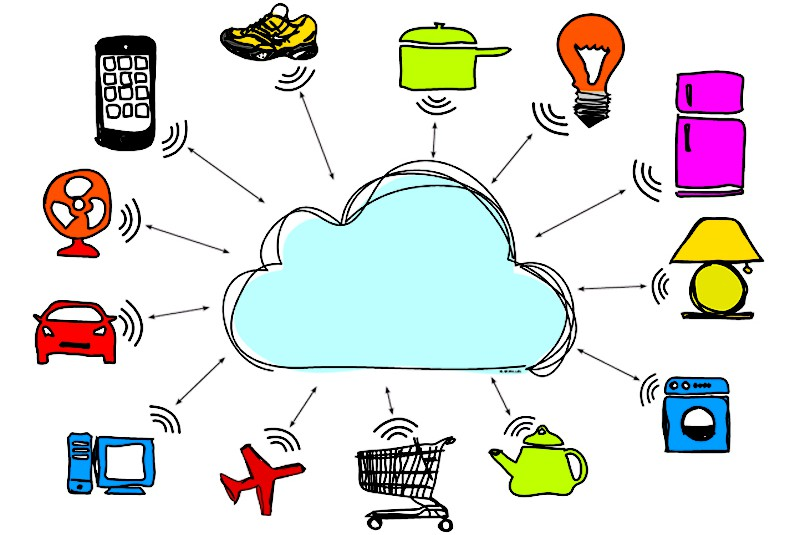
\includegraphics[width=.6\textwidth]{things.jpg}\footnotemark
	\end{figure}
	
	\footnotetext{https://www.codeproject.com/KB/Wearables/831012/}
\end{frame}

\begin{frame}{}	
	\begin{block}{Internet das Coisas}		
		O termo foi criado por Kevin Ashton, a um pioneiro tecnológico britânico que concebeu um \textbf{sistema de sensores onipresentes} conectando o mundo físico à Internet, enquanto trabalhava em identificação por rádio frequência (RFID) \cite{Amazon}.\\ 
		\vspace{4pt}
		\textbf{Em resumo:} são dispositivos \textbf{que falam entre si} sem intervenção humana.
	\end{block}
	
	\begin{figure}[H]
		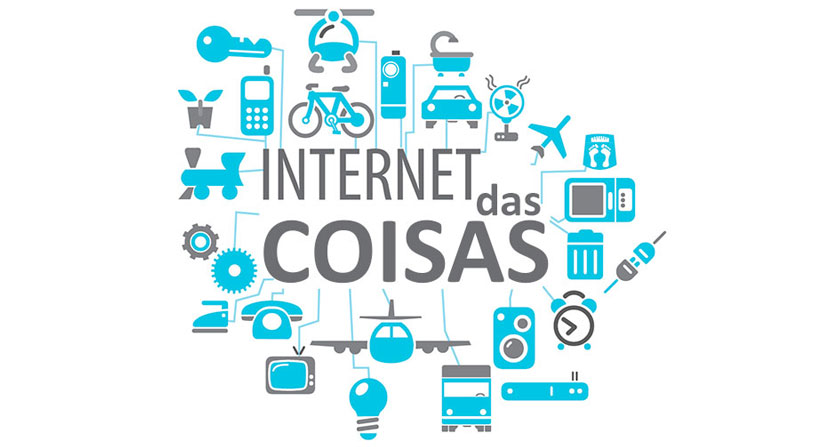
\includegraphics[width=.6\textwidth]{ioc.jpg}\footnotemark
	\end{figure}
	
	\footnotetext{http://www.blogindustrial.com.br/wp-content/uploads/2016/12/}
\end{frame}

\subsection*{Características}
\begin{frame}{}
	\begin{block}{}	
		As \textbf{coisas}, a \textbf{Internet} e a \textbf{conectividade} são os três componentes principais da IoT, mas o seu valor está no fechamento das \textbf{lacunas entre os mundos físico e digital} em sistemas com recursos de reforço e aprimoramento automáticos \cite{Amazon}.
		\begin{itemize}
			\item A coisa tem que ser \textbf{única};
			\item Deve realizar processamento/\textbf{análise} de dados;
			\item Precisa \textbf{comunicar-se} com outra(s) coisa(s);
			\item Precisa ser \textbf{controlada}\footnotemark remotamente.
		\end{itemize}
	\end{block}
	
	\footnotetext{Comandar, medir, telemetrar ou gerenciar.}
\end{frame}